\begin{activity} \label{A:11.6.4} Consider the cylinder with radius $a$ and height $h$ defined parametrically by
\[\vr(s,t) = a\cos(s) \vi + a\sin(s) \vj + t \vk\]
for $0 \leq s \leq 2\pi$ and $0 \leq t \leq h$, as shown in Figure \ref{F:11.6.SA_cylinder_ex}.
\begin{figure}[h]
\begin{center}
%\resizebox{!}{2.0in}{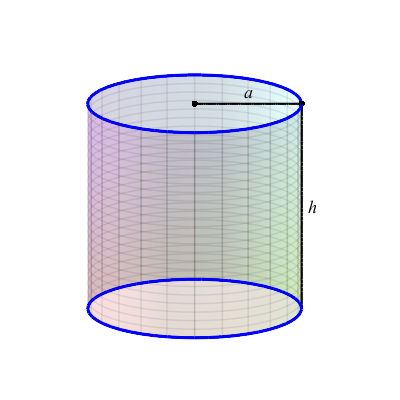
\includegraphics[trim=2cm 2cm 2cm 2cm, clip]{11_6_SA_cylinder}}
  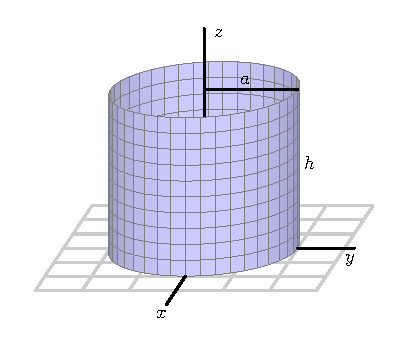
\includegraphics{figures/fig_11_6_cylinder.eps}
\end{center}
\caption{A cylinder.}
\label{F:11.6.SA_cylinder_ex}
\end{figure}
	\ba
	\item Set up an iterated integral to determine the surface area of this cylinder.
	
	\item Evaluate the iterated integral. 
	
	\item Recall that one way to think about the surface area of a cylinder is to cut the cylinder horizontally and find the perimeter of the resulting cross sectional circle, then multiply by the height.  Calculate the surface area of the given cylinder using this alternate approach, and compare your work in (b).

	\ea

\end{activity}
\begin{smallhint}

\end{smallhint}
\begin{bighint}

\end{bighint}
\begin{activitySolution}
\ba
\item We have 
\[\vr_s(s,t) = -a\sin(s) \vi + a\cos(s) \vj  \ \text{ and } \ \vr_t(s,t) = \vk,\]
so the area of the surface of the cylinder is 
\[\int \int_D |\vr_s \times \vr_t| \, dA = \int \int_D a \, dA.\]
In this case, $dA = ds \ dt$, so an iterated integral that represents the area of the surface is 
\[\int \int_D |\vr_s \times \vr_t| \, dA = \int_{0}^{h} \int_{0}^{2 \pi} a \, ds \, dt.\]

\item We can find the surface area of the cylinder by multiplying the circumference of the circle of radius $a$ by the height $h$ to obtain $2 \pi a h$. Evaluating the iterated integral yields
\begin{align*}
\int_{0}^{h} \int_{0}^{2 \pi} a^2 \, ds \, dt &= a \int_{0}^{h} \left. s \right|_{0}^{2 \pi}  \, dt \\
	&= 2 \pi a \int_{0}^{h}  \, dt \\
	&= 2 \pi a \left. t \right|_{0}^{h}  \\
	&= 2 \pi a h.
\end{align*}

\item If we slice the cylinder horizontally, a cross section is a circle of radius $a$. The circumference of this circle is $2 \pi a$. We multiply by the height of the cylinder to obtain the surface area as $2 \pi a h$ as expected. 
\ea
\end{activitySolution}
\aftera

